\subsection{Overview}
\begin{figure}[h!]
	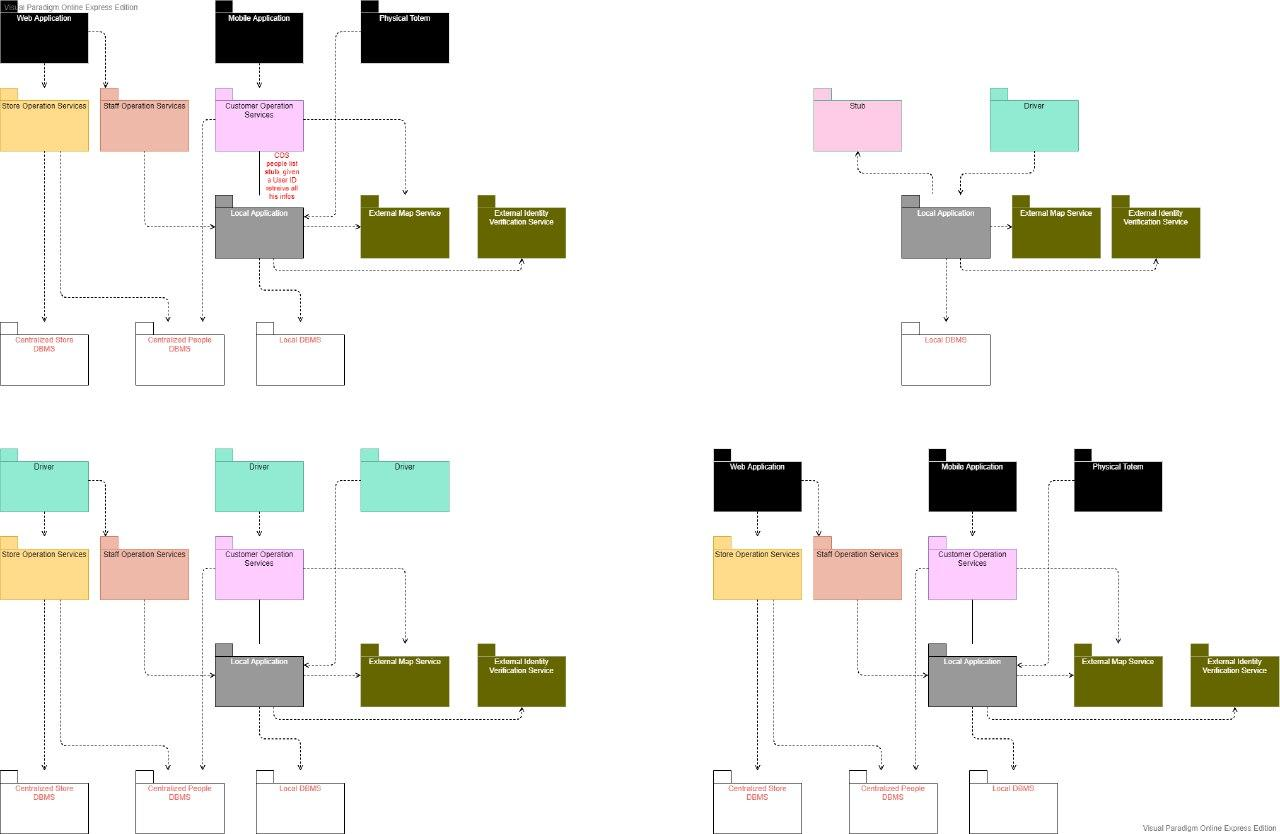
\includegraphics[width=\linewidth]{../Diagrams/Implementation.png}
	\caption{Implementation}
	\label{fig:Implementation1}
\end{figure}
In this part there will be an explanation on how and in which order the development, integration and testing of this project should be done. The idea is to complete a end user testable version with the bare minimum functionalities as soon as possible so that then it is possible to test this base extensively while adding the rest of the features.
\subsection{Implementation Plan}
The chosen approach for implementing, testing and integrating the system is a combination of bottom-up and threads given the limited number of complex components that compose it.
This way it is in fact possible to firstly develop completely and properly test the core functionality, which is the virtual queuing on the user part, and then add the other functionalities i.e. booking the entrance on a certain time and date (which can partially be seen as an extension of the virtual queuing), ordered stores suggestions given filters and current queues and lastly the store management functions on the store manager’s part.\\
The aim of this approach is to implement, integrate and test an initial version of all the components as soon as possible so that then the missing features can be developed on a functioning base with the minimum need of drivers and stubs and by keeping them simple when they are strictly needed.
Thus the development of each component will be incremental once an initial version of the system with basic features from start to end is finished.\\

The threads approach anyway has to be guided by the bottom-up one because there are some dependencies between the components.\\

The development has to start with the \textbf{Local DBMS} and \textbf{Local Application} component (an instance of it will be hosted by every registered store) which is the core of the management of information about queues, bookings, user reports and user notifications, and practically feeds the CLup system and clients with operational information. For now only the queues and notifications subcomponents will be developed according to the threads approach. Also the interface with the physical totems will be developed in order to allow people to queue in the stores even if they don’t use the client application, which is part of the basic functionality. At this stage the \textbf{external components} will be connected to the system, they will not require any testing on their own since they come from sources that are assumed trustable and reliable.

After this the development of three more components can start: on the store side \textbf{Staff Operation Services}, which is needed for the functioning of the web app’s control panel available to the store managers, for now only its functionality to allow and stop store entrances will be developed; on CLup’s server side the components \textbf{Store Operation Services} together with \textbf{Centralized Store and People DBMSs} and \textbf{Customer Operation Services} can be developed, the former in its entirety while the latter only with the functionalities that can already be integrated and tested according to what was developed in Local Application (e.g. no booking management).\\

Now it is possible to develop the user interfaces for each module: the \textbf{Mobile Application} for the smartphone users, the \textbf{Web Application} for the store managers and the \textbf{Physical Totem} software for those who don’t use the application. For each of these interfaces (for now) it’s enough to implement interactions just for those functions of the system that have already been developed.\\

After these steps there should be a functioning system composed of a mobile application, a program to be installed on store servers, a program to be deployed on physical totems and a system to be used on the main CLup servers to allow interactions between the previous: with these you should be able to accomplish basic tasks objective of the scope of this project such as register users, stores, do logins, get tickets to virtually queue in stores and enter and exit them with such tickets. The testing can then proceed over this basic version of CLup while the development keeps going on by implementing the missing features described in the RASD: the possibility for users to book entrances, algorithms to properly sort and suggest stores and times to go shopping and the remaining functions for the store manager’s web app.
Component wise the method to use in order to implement these features is the same as the one previously described, and still in a thread manner if needed because of developers’ availability.
Summing up the implementation order goes in 3 phases with respective components: \begin{enumerate}
	\item The stores’ local application: Local DBMS and Local Application
	\item Central CLup system and local store interaction with this system: Staff Operation Services, Store Operation Services, Customer Operation Services, Centralized People and Centralized Store DBMSs
	\item The users and store staff interfaces: Web Application, Mobile Application and Physical Totem
\end{enumerate}




\subsection{Integration Strategy}
The integration of the components follows their implementation, so that no components will remain isolated at any time during development in order to avoid the risk of inconsistencies between them.
\begin{enumerate}
	\item In a first moment the Local DBMS and Local Application are integrated, also the two external components are integrated in the system. A stub and a driver are used to simulate the components supposed to interact with the local application, anyway they don’t need to be complex at all since all that is being implemented and integrated for now is just the basic functionalities and subcomponents, so Bookings and Reports will be left out for now.
	\begin{figure}[H]
		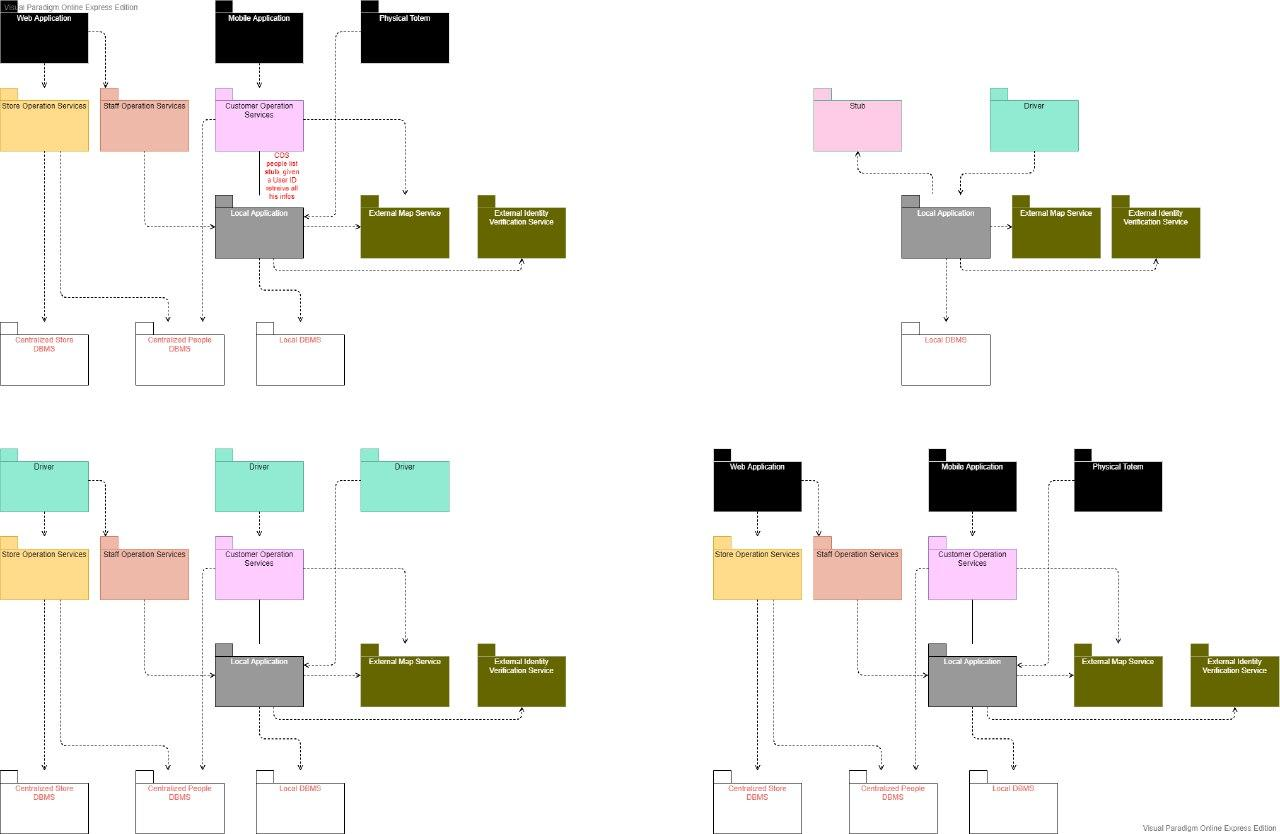
\includegraphics[width=\linewidth]{../Diagrams/Implementation.png}
		\caption{Implementation}
		\label{fig:Implementation2}
	\end{figure}
	\item Now Staff Operation Services is integrated with local application, also Store Operation Services (with its DBMSs) comes into the picture since they both share a Driver for the Web Application. The other part of the central CLup’s system can also be integrated since Local Application is ready: Customer Operation Services, there will be a driver for this part representing the mobile app and also a driver for the totem will remain from the previous step.
	\begin{figure}[H]
		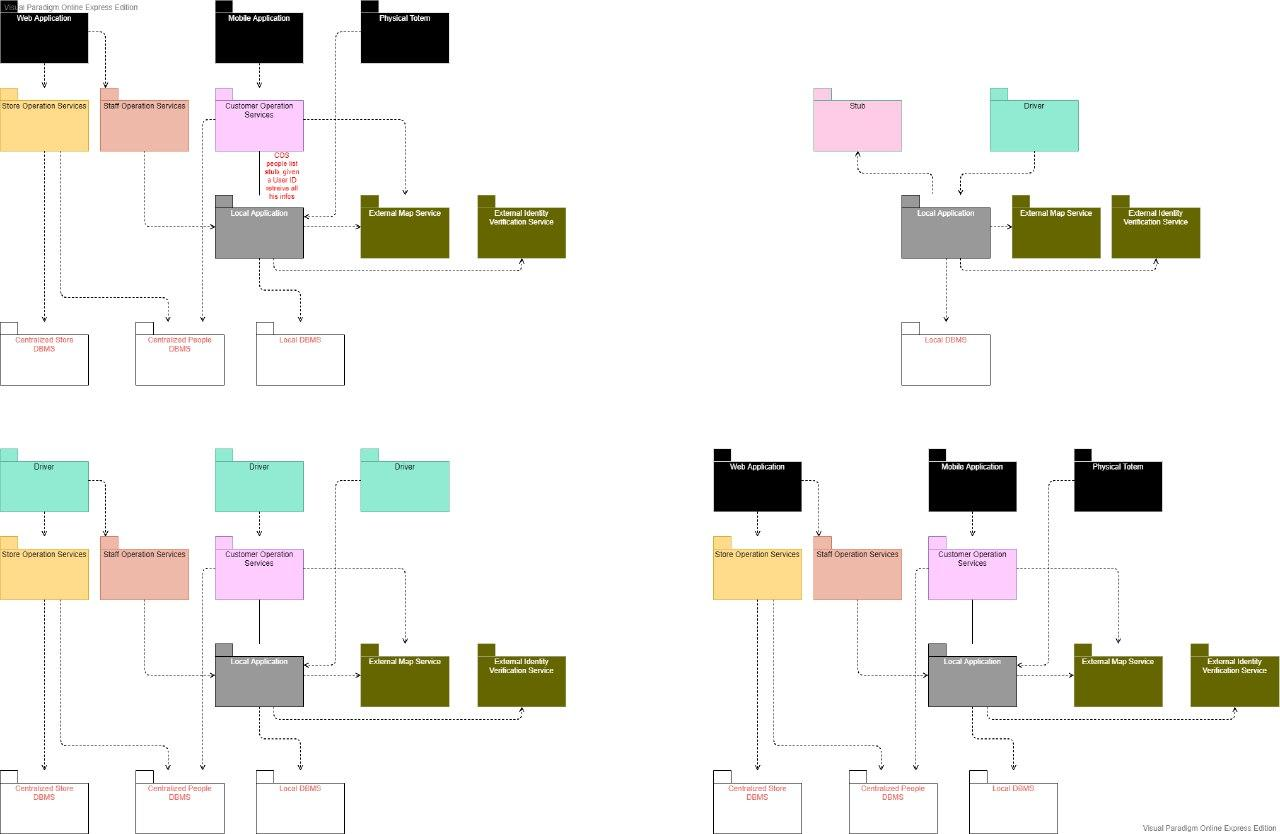
\includegraphics[width=\linewidth]{../Diagrams/Implementation.png}
		\caption{Implementation}
		\label{fig:Implementation3}
	\end{figure}
	\item Lastly the user interfaces are integrated in order to complete the initial version of the project, now the remaining sub components will integrated following the order in which their respective components were integrated explained in this section.
	\begin{figure}[H]
		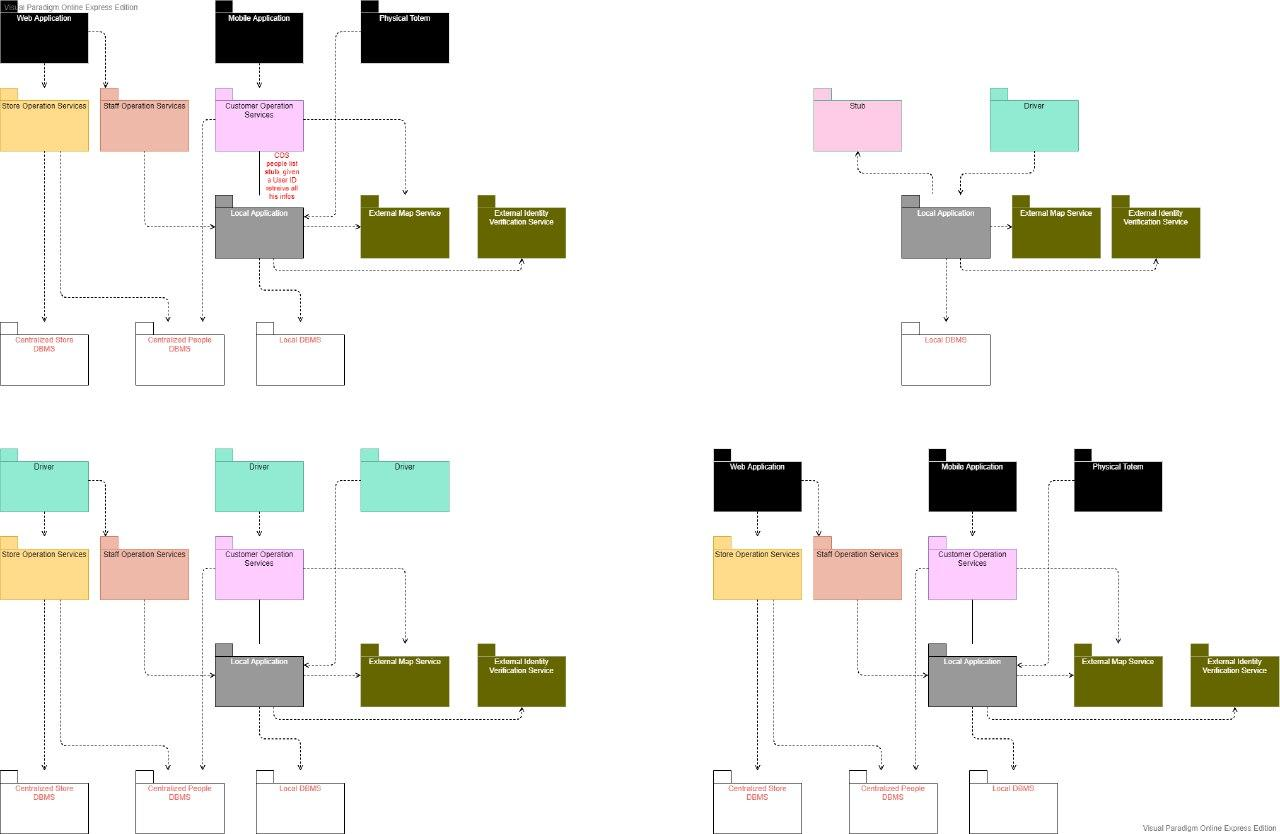
\includegraphics[width=\linewidth]{../Diagrams/Implementation.png}
		\caption{Implementation}
		\label{fig:Implementation4}
	\end{figure}
\end{enumerate}

\subsection{System Testing}
Upon the completion of the basic version of the system, again at the completion of each system feature, and most importantly after the implementation and integration of every feature, the system must be tested on its entirety. The tests are meant to verify the satisfaction of both functional and non functional requirements.

\subsection{Additional Specification on Testing}